\documentclass[12pt, letterpaper]{article}
\usepackage[utf8]{inputenc}
\usepackage{indentfirst}
\usepackage{graphicx}
\usepackage{setspace}
\usepackage[numbers]{natbib}
\usepackage [autostyle, english = american]{csquotes}
\MakeOuterQuote{"}
\usepackage{layout}
\usepackage[title]{appendix}
\usepackage[justification=centering]{caption}
\usepackage{titlesec}
\usepackage[percent]{overpic}
\usepackage{amsmath}
\usepackage{systeme}
\usepackage{blkarray, bigstrut}
\usepackage{tikz}
\usetikzlibrary{tikzmark}
\usepackage[utf8]{inputenc}
\usepackage{relsize}
\usepackage[nameinlink, capitalize, noabbrev]{cleveref}
\usepackage{tabu}

\setlength\parskip{\baselineskip}

%prevent hyphenation of words
\emergencystretch=\maxdimen
\hyphenpenalty=10000
\hbadness=10000

\begin{document}

\setcounter{secnumdepth}{-1}
\titlespacing*{\section}{0pt}{1.5\baselineskip}{.25\baselineskip}
\binoppenalty=\maxdimen
\relpenalty=\maxdimen

\setlength{\abovedisplayskip}{-0.5\baselineskip}
\setlength{\belowdisplayskip}{0\baselineskip}
\setlength{\abovedisplayshortskip}{0\baselineskip}
\setlength{\belowdisplayshortskip}{0\baselineskip}

%Cover page: 5pts
%Course, subject, name, date
\title{MA348 Numerical Analysis, Integration}
\author{David Jefts}
\date{April 24\textsuperscript{th}, 2019}
\begin{titlepage}
	\centering
	\maketitle
	\centering
	\hfill
	\vfill
	\thispagestyle{empty}
\end{titlepage}

\setlength{\voffset}{-0.5in}
\setlength{\headsep}{10pt}

%Introduction: 5pts
%Describe the problem and state objectives
\section{\label{sec:intro}Introduction}
	%Lab9: Use the trapezoid rule ( with 2, 4 and 6 intervals) , the Simpson rule( with 5 points) and the Gaussian quadrature with 2 points to approximate : the integral of f between 0 and 0.8, where f(x)=0.2+25x-200x^2+675x^3-900x^4+400x^5
	The purpose of this lab is to use compare the effectiveness of different algorithms at estimating the value of an integral, $\displaystyle\int_{a}^{b}\!{f(x)}\,\mathrm{d}x$, where $a$ is 0, $b$ is 0.8, and $f(x)={0.2+25x-200x^2+675x^3-900x^4+400x^5}$.
	
	$\displaystyle\int_{0.0}^{0.8}\!{0.2+25x-200x^2+675x^3-900x^4+400x^5}\,\mathrm{d}x$
	 
	 The three methods used to solve the above definite integral were the Newton-Cotes Trapezoidal Method, the Newton-Cotes Simpson method, and the Gaussian Quadrature method. The Trapezoid method was used with 2-, 4-, and 6-subintervals, the Simpson method was used with five subintervals, and the Gaussian Quadrature was used with two subintervals.

%Theory-Analysis: 5pts
%State assumptions and develop equations
\section{\label{sec:theory}Theory-Analysis}
	
	
	In this lab I made the assumption that the actual value of the integral is 1.640533333.

	 
%Numerical Solution: 20pts
%Describe the numerical methods used to solve the problem
\section{\label{solution}Numerical Solution}
	All three integration methods were coded in Python, with this report created in \LaTeX{}.
	
	The Newton-Cotes Trapezoidal method is a method of integration based upon breaking up the integral into multiple subintervals and then drawing trapezoids that estimate the area under the function curve, as shown below:
	
	\begin{figure}[h]
            		\centering
            		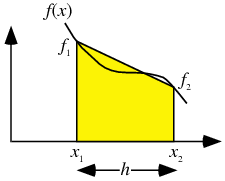
\includegraphics[width=0.5\linewidth]{trapezoid.png}
            	\end{figure}
	
	 \newpage$f(x)$ is the function line, $h$ is the width of each subinterval (also known as the $\delta x$), $x_1$ and $x_2$ are the endpoints of the subinterval and $f_1$ and $f_2$ are the corresponding function values. The yellow area is the trapezoid that represents the integral estimation for that subinterval and is represented by:
	 
	 \begin{equation*} I = \frac{h}{2} \left[f(x_0)+2\sum_{i=1}^{n-1}{f(x_i)}+f(x_n)\right] \end{equation*}
	 
	 This is a summation of all of the trapezoids between each limit of the integral when there is $n$ subintervals with each $x$ value representing the vertical lines dividing the subintervals.
	 
	 The Simpson formula is very similar to the Trapezoidal formula, except that it uses the midpoint of each subinterval as well as the end points when estimating the integral value.
	 
	 \begin{equation*} I = \frac{h}{3} \left[f(x_0)+4\!\!\!\sum_{i=1, 3, 5...}^{n-1}{\!\!\!f(x_i)}+2\!\!\!\sum_{i=2, 4, 6...}^{n-1}{\!\!\!f(x_i)}+f(x_n)\right] \end{equation*}
	 
	 The Gaussian Quadrature method is slightly different from the other integration methods. It only works on the interval $[-1, 1]$ and adds constraints on the integral equation to reduce the error. This method assumes that there will be zero integration error if, and only if, the following four conditions are met on the integral of $f(x)$ from -1 to 1:
	 
	 \begin{enumerate}
	 \item \begin{equation*}f=1::\int_{-1}^{1}{1\mathrm{d}x}=2=c_0f(x_0)+c_1f(x_1)=c_0+c_1\end{equation*}
	 \item \begin{equation*}f=x::\int_{-1}^{1}{x\mathrm{d}x}=0=c_0x_0+c_1x_1\end{equation*}
	 \item \begin{equation*}f=x^2::\int_{-1}^{1}{x^2\mathrm{d}x}=\frac{2}{3}=c_0x_0^2+c_1x_1^2\end{equation*}
	 \item \begin{equation*}f=x^3::\int_{-1}^{1}{x^3\mathrm{d}x}=0=c_0x_0^3+c_1x_1^3\end{equation*}
	 \end{enumerate}
	 
	 These equations can be used to make the following:
	 
	 \begin{equation*}x_0=-x_1\quad \text{by symmetry}\end{equation*}
	 \begin{equation*}c_0=c_1\end{equation*}
	 \begin{equation*}\frac{2}{3}=2x_0^2 \quad\rightarrow\quad x_0=\pm\sqrt{\frac{1}{3}}\end{equation*}
	 \begin{equation*}x_0=\sqrt{\frac{1}{3}}\quad\quad x_1=-\sqrt{\frac{1}{3}}\end{equation*}
	 
	 These, in turn, all lead to the full integral equation that we actually care about:
	 
	 \begin{equation*}\int_{-1}^{1}{f(x)\mathrm{d}x}=f\left(-\frac{1}{\sqrt{3}}\right)+f\left(\frac{1}{\sqrt{3}}\right)\end{equation*}
	 
	However this only works on that specific integral and the integral that is being solved must be morphed so that it's limits of integration match $[-1,1]$.


%Results and Discussion: 45pts
%Tabulate and plot the results, compare results, and discuss the accuracy of results
\section{\label{sec:results}Results and Discussion}
    	The table of the divided differences values and coefficients (rounded to four decimal places) as described in the Numerical Solution Section is shown below:
	
	\begin{table}[h]
	\centering
	\begin{tabular}{>{$}c<{$} >{$}c<{$} >{$}c<{$} >{$}c<{$} >{$}c<{$}}
	x \text{ input} & \text{DD 1} & \text{DD 2} & \text{DD 3} & \text{DD 4}\\
	1.0 & 0.0 &&&  \\
	&& [y_0, y_1]=0.4621 && \\
	4.0 & 1.3863 && [y_0, y_1, y_2]=-0.1969 \\
	&& [y_1, y_2]=-0.3254 & & [y_0, y_1, y_2, y_3]=0.1450 \\
	5.0 & 1.0609 && [y_0, y_1, y_2]=0.5281 \\
	&& [y_2, y_3]=0.7308 && \\
	6.0 & 1.7918 &  &  \\
	\end{tabular}
	\end{table}
	
	The final polynomial is therefore:
	
	\begin{equation*}
	f(x) = 0.4102249 + 0.3285789(x-1.0) + 0.0189155(x-1.0)(x-4.0) + 0.0078654(x-1.0)(x-4.0)(x-5.0)
	\end{equation*}
	
	Simplified:
	
	\begin{equation*}
	f(x) = 0.0078654x^3 - 0.0597385x^2 + 0.462098x + 0
	\end{equation*}
	%$(C)x^3+(-B-10C)x^2+(A+5B+29C)x+(-A+4B-20C)$
	\newpage
	Below is the graph of the interpolated polynomial, the initial input coordinates, and the estimated value for ln(2):
%	\begin{figure}[htp]
%            			\centering
%            			\includegraphics[width=1.0\linewidth]{}
%            		\end{figure}
	


%Conclusions: 20pts
%Comment on the efficiency of the solvers
\section{\label{conclusion}Conclusions}
	The Newton Divided Differences method is very effective at interpolating functions from a set of points, however the results from this lab may have been much more accurate with the utilization of more input coordinates. Additionally, this method seems to require a degree of precision not always possible with some modern calculators and computers. In conclusion, the Newton Divided Differences Interpolation Method is effective at estimating function. curves, but it requires a significant amount of points to increase its accuracy. 

\pagebreak
%Appendices
%Include listings of the source codes, include printed copies of the output files
\appendix
%	\section{Appendix A}
%            	\begin{figure}[h]
%            		\centering
%            		\includegraphics[width=1.0\linewidth]{}
%            	\end{figure}
%		
%	\newpage
%	\section{Appendix B}
%            	\begin{figure}[h]
%            		\centering
%            		\includegraphics[width=.8\linewidth]{}
%            	\end{figure}
		
		
		


\end{document}
